\pdfoutput=1
\documentclass[preview]{standalone}

\usepackage[utf8]{inputenc}
\usepackage{lmodern}
\usepackage[T1]{fontenc}

\usepackage{verbatim}
\usepackage{graphicx}
	\DeclareGraphicsRule{*}{mps}{*}{}
\usepackage{xcolor}

\usepackage{tikz}
	\usetikzlibrary{calc}
	\usetikzlibrary{arrows}
	\usetikzlibrary{backgrounds}
	\usetikzlibrary{decorations.pathmorphing}
	\usetikzlibrary{shapes.geometric}
	\tikzset{>=latex'}

\usepackage{amsmath}
\usepackage{amssymb}
\usepackage{dsfont}
\usepackage{nicefrac}
\usepackage{mathrsfs}
\usepackage[Euler]{upgreek}
\usepackage[nointegrals]{wasysym}
\usepackage{booktabs}
\usepackage{float}

\begin{document}

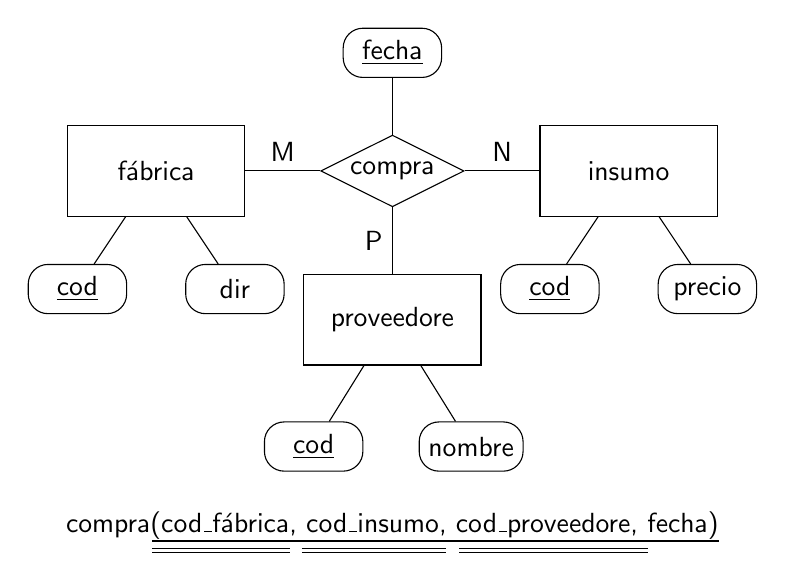
\begin{tikzpicture}[font=\sffamily]
	\node[draw,minimum width=2.25cm,minimum height=1.15cm] (ent1) at (0,0) {fábrica};
	\node[draw,minimum width=2.25cm,minimum height=1.15cm] (ent2) at (6,0) {insumo};
	\node[draw,minimum width=2.25cm,minimum height=1.15cm] (ent3) at (3,-1.89) {proveedore};
	\node[draw,shape aspect=2,diamond,inner sep=0.5mm] (rel) at (3,0) {compra};
	\draw (ent1) -- node[above]{M} (rel) -- node[above]{N} (ent2) (rel) -- node[left]{P} (ent3);
	\node[draw,rounded corners=2.5mm,minimum width=1.25cm,minimum height=6.25mm] (ent1 id) at (-1,-1.5) {$\underline{\text{cod}}$};
	\node[draw,rounded corners=2.5mm,minimum width=1.25cm,minimum height=6.25mm] (ent1 dir) at (1,-1.5) {dir};
	\node[draw,rounded corners=2.5mm,minimum width=1.25cm,minimum height=6.25mm] (ent2 id) at (5,-1.5) {$\underline{\text{cod}}$};
	\node[draw,rounded corners=2.5mm,minimum width=1.25cm,minimum height=6.25mm] (ent2 precio) at (7,-1.5) {precio};
	\node[draw,rounded corners=2.5mm,minimum width=1.25cm,minimum height=6.25mm] (ent3 id) at (2,-3.5) {$\underline{\text{cod}}$};
	\node[draw,rounded corners=2.5mm,minimum width=1.25cm,minimum height=6.25mm] (ent3 nombre) at (4,-3.5) {nombre};
	\node[draw,rounded corners=2.5mm,minimum width=1.25cm,minimum height=6.25mm] (rel fecha) at (3,1.5) {$\underline{\text{fecha}}$};
	\draw (ent1)--(ent1 id);
	\draw (ent1)--(ent1 dir);
	\draw (ent2)--(ent2 id);
	\draw (ent2)--(ent2 precio);
	\draw (rel)--(rel fecha);
	\draw (ent3)--(ent3 id);
	\draw (ent3)--(ent3 nombre);
	\node (compra rel) at (3,-4.5) {compra(cod\_fábrica, cod\_insumo, cod\_proveedore, fecha)};
	\draw (-0.05,-4.70)--(7.15,-4.70);
	\draw (-0.05,-4.80)--(1.70,-4.80);
	\draw (-0.05,-4.85)--(1.70,-4.85);
	\draw (1.85,-4.80)--(3.68,-4.80);
	\draw (1.85,-4.85)--(3.68,-4.85);
	\draw (3.85,-4.80)--(6.25,-4.80);
	\draw (3.85,-4.85)--(6.25,-4.85);
\end{tikzpicture}

\vskip 2pt

\sffamily
fábrica(\underline{cod}, dirección) \quad insumo(\underline{cod}, precio) \quad proveedore(\underline{cod}, nombre)\\

\end{document}
